\documentclass[a4paper]{article}
\usepackage{ucs}  % unicode
\usepackage[utf8x]{inputenc}
\usepackage{multirow}
\usepackage{array}
% \usepackage[T2A]{fontenc}
% \usepackage[bulgarian]{babel}
\usepackage{graphicx}
\usepackage{subfig}
% \usepackage{fancyhdr}
% \usepackage{lastpage}
\usepackage{listings}
\usepackage{amsfonts}
\usepackage{amsmath}
% \usepackage{fancyvrb}
\usepackage[usenames,dvipsnames]{color}
% \setlength{\headheight}{12.51453pt}

%\pagestyle{fancy}
%\fancyhead{}
%\fancyfoot{}

% \cfoot{\thepage\ от \pageref{LastPage}}

% \addto\captionsbulgarian{%
%   \def\abstractname{%
%     Цел на проекта} %\cyr\CYRA\cyrs\cyrt\cyrr\cyra\cyrk\cyrt}}%
% }

% Custom defines:

% TODO remove colorlinks before printing
\usepackage[unicode,colorlinks]{hyperref}   % this has to be the _last_ command in the preambule, or else - no work
\hypersetup{urlcolor=blue}
\hypersetup{citecolor=PineGreen}

\def\d{\mathrm{d}}

\begin{document}

\title{Pedestrian detection and leg pose estimation \\
       High Level Computer Vision - Final Project Report}
\author{Zornitsa Kostadinova \\ Iskren Ivov Chernev}
\maketitle

\begin{abstract}
The purpose of this report is to present a simple algorithm for pedestrian
detection and leg position estimate and provide performance results.
\end{abstract}
\newpage

\section{Introduction}
Pedestrian detection and pose estimate are well known problems in computer
vision with numerous application in many areas. The algorithm presented in this
report does not provide state-of-the-art performance, but instead is a base
line approach using well established tools to provide an estimate of what can
be expected from bare application of standard tools for the task.

\section{Related work}
The algorithm presented here is using the hessian \cite{hessian} interest point
detector, combined with SIFT \cite{sift} \cite{sift2} interest point
descriptors. It uses k-means to cluster the point descriptors \cite{kmeans}.
Then it records appearance information about each cluster to use when matching.
This technique is known as the Implicit Shape Model \cite{ism}. For the exact
localization of the pedestrian a generalized hough transform is applied
\cite{hough}. After a pedestrian bounding box is detected a HOG descriptor is
computed \cite{hog1}, and a SVM regression is performed to guess the joint
positions of the ankle and knee of both legs \cite{svm1}.

\section{Method}
The algorithm is composed of two stages, pedestrian detection (side views only)
and leg position estimate.

Detection training is performed by first finding interest points using Hessian
detector.  Then SIFT descriptor is computed and the descriptors are clustered
using k-means. Next all points are matched to all cluster centers, and under
a certain threshold, are recorded as appearance information for that cluster,
containing the offset to the center of the object.

Detection testing includes finding the interest points in the test image (again
with Hessian), computing their SIFT descriptors and matching them to the
cluster centers. The interest points vote for the occurrences of each of the
clusters they match (under certain threshold). The vote space (in this case
only X, Y) is then smoothed with Gaussian and only the local maximums are taken
into account. In this algorithm the first match is considered to contain
a pedestrian, and all other (having lower score) matches are discarded.
Bounding box is formed by taking the object center and fitting a fixed size box
around it. The size of the box is computed by averaging the width and height of
all training bounding boxes.

Leg pose estimation training is performed by examining annotated data
containing joint positions of pedestrians and computing the angle that each
joint forms with the $ Ox\vec{} $ axes. The bounding box is normalized to
a fixed size for all training data and then its HOG feature descriptor is
computed using \cite{hogImp}. 4 different SVMs are trained to guess each joint
angle given the HOG descriptor (SVM regression, using \cite{svmToolkit}).

Leg pose estimation testing is performed by taking a bounding box of
a suspected pedestrian (either from annotations or output from the detection
stage), computing its HOG descriptor and multiplying it with the SVM model
created in the training phase. Then the mean of the distance between joints
(thigh and leg lengths) and triangulation is performed to estimate the actual
positions of the joints given the angles.

\section{Experiments}
The detection and pose estimation phase were tested both independently and
together. A total of 210 images were used, separated in two groups of around
100, training on one group and then testing on the other. The reason for this
is that the background of the images was similar in each group so the training
would be biased if the test examples contained images with the same
background/person.

Detection accuracy is computed by the number of correctly located pedestrians,
because we assume there is exactly only one pedestrian in the image. The
average accuracy for this phase is 49\%. Accuracy can further be improved by
fine tuning all the available parameters, but this was not done, because of the
lengthy testing phase and the limited available time.
 
\begin{figure}[h!]
  \centering
  \subfloat[Smoothened hough voting space]{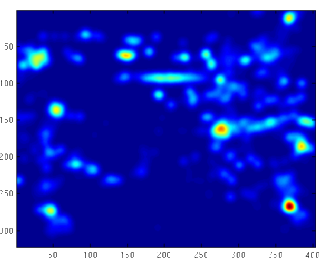
\includegraphics[width=0.5\textwidth]{hough.png}}                
  \subfloat[Activated points and detections]{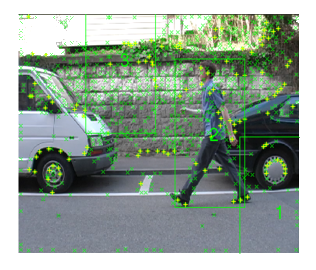
\includegraphics[width=0.5\textwidth]{ism1.png}}
  \caption{Detection phase}
  \label{fig:detection}
\end{figure}

Pose estimation accuracy was measured by the L2 distance of the real joint
angles vector and the guessed angle vector. The average accuracy was 0.11
(smaller is better). Visualization further approved the fact that the detection
was actually pretty accurate.

\begin{figure}[h!]
  \centering
  \subfloat[Accuracy distribution]{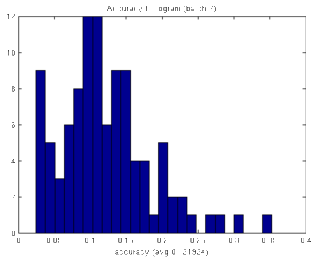
\includegraphics[width=0.5\textwidth]{pose_acc.png}}                
  \subfloat[Pose estimate and ground truth]{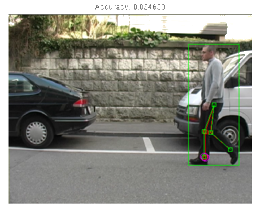
\includegraphics[width=0.5\textwidth]{pose1.png}}
  \caption{Pose estimation phase}
  \label{fig:pose_estimate}
\end{figure}

Pose estimation was performed both on its own and on output from the detection
phase. Surprisingly the accuracy was roughly the same, regardless of the fact
that the detection phase was sometimes giving not very well placed bounding
boxes.

\begin{figure}[h!]
  \centering
  \subfloat{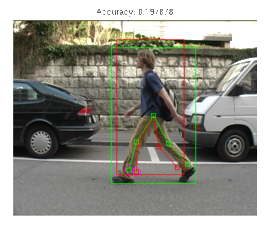
\includegraphics[width=0.5\textwidth]{full1.png}}                
  \subfloat{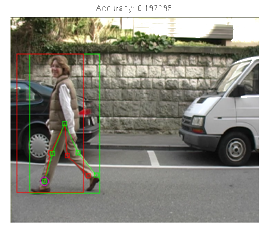
\includegraphics[width=0.5\textwidth]{full2.png}}
  \caption{Detection and estimation combined}
  \label{fig:detection_estimation}
\end{figure}

\section{Conclusions}
The techniques used for detection were very powerful and much more can be
squeezed out by carefully altering the parameters. The most important ones
turned out to be codebook size (number of clusters), thresholds for matching
the codebook and smoothing the hough space with Gaussian, instead of just using
square buckets.

The HOG + SVM seems to need less care, in terms of altering parameters (it
doesn't have any), and it actually performed pretty well during
experimentation. Further improvements might come out of using structured
regression SVM, that is, one that uses the relationship between different
joints instead of guessing all of them independently. Different representation
of the joints may also be profitable -- one can add lengths of thigh and leg to
the angles or use $ (x, y) $ coordinates.

In case of continuous frames information can be shared between frames to
further improve the accuracy. Also from joint positions one can easily compute
a ``walking cycle'' position -- that is a real from $ [0, 1] $ representing the
position in a walking cycle of positions -- from legs fully spread, to legs
next to each other or something similar.

\begin{thebibliography}{99}
  \bibitem{hog1} Navneet Dalal, Bill Triggs, "Histograms of Oriented Gradients for Human Detection," cvpr, vol. 1, pp.886-893, 2005 IEEE Computer Society Conference on Computer Vision and Pattern Recognition (CVPR'05) - Volume 1, 2005
  \bibitem{hogImp} HOG implementation taken from \url{http://people.cs.uchicago.edu/~pff/latent/}
  \bibitem{svm1} Vladimir Vapnik. The Nature of Statistical Learning Theory. Springer-Verlag, 1995. ISBN 0-387-98780-0.
  \bibitem{svmToolkit} SVM toolkit homepage \url{http://www.isis.ecs.soton.ac.uk/resources/svminfo/}
  \bibitem{ism} Leibe, Bastian; Leonardis, Ales; Schiele, Bernt; An Implicit
                Shape Model for Combined Object Categorization and
                Segmentation; 2006, Springer
  \bibitem{sift} Distinctive Image Features from Scale-Invariant Keypoints; David G. Lowe; 2004
  \bibitem{sift2} Object Recognition from Local Scale-Invariant Features; David G. Lowe; 1999
  \bibitem{hessian} Mikolajcyk, K. and Schmid, C. 2002. An affine invariant
                    interest point detector. In Proceedings of the 8th
                    International Conference on Computer Vision, Vancouver,
                    Canada
  \bibitem{kmeans} Steinhaus, H. (1956). "Sur la division des corps matériels
                   en parties" (in French). Bull. Acad. Polon. Sci. 4 (12):
                   801–804. MR0090073.  Zbl 0079.16403.
  \bibitem{hough} D.H. Ballard, "Generalizing the Hough Transform to Detect
                  Arbitrary Shapes", Pattern Recognition, Vol.13, No.2,
                  p.111-122, 1981
\end{thebibliography}

\end{document}
